\documentclass{standalone}
\usepackage{tikz}
\usepackage{ctex,siunitx}
\usepackage{tkz-euclide}
\usepackage{amsmath}
\usetikzlibrary{patterns, calc}
\usetikzlibrary {decorations.pathmorphing, decorations.pathreplacing, decorations.shapes,}
\begin{document}
\small
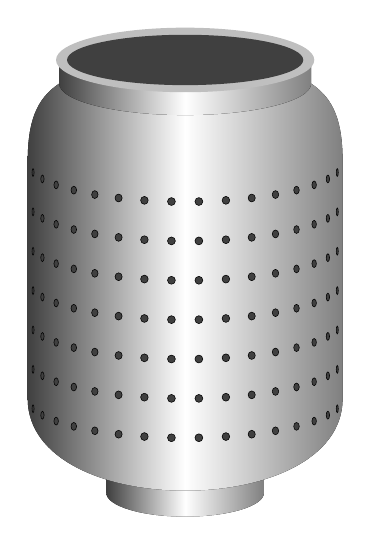
\begin{tikzpicture}[>=latex,scale=1]
  % \useasboundingbox(,)rectangle(,);
  \fill[left color=darkgray,right color=gray,middle color=white](-1,1)--(-1,-0.2)arc(-180:0:1 and 0.3)--(1,1);
  \fill[left color=darkgray,right color=gray,middle color=white](-1.6,5)..controls(-1.9,4.8)and(-2,4.5)..(-2,4)--(-2,1)to[bend right=90](2,1)--(2,4)..controls(2,4.5)and(1.9,4.8)..(1.6,5);
  \fill[left color=darkgray,right color=gray,middle color=white](-1.6,5.3)--(-1.6,5.0)arc(-180:0:1.6 and 0.4)--(1.6,5.3)--cycle;
  \fill[lightgray](0,5.3)ellipse(1.64 and 0.41);
  \fill[darkgray](0,5.3)ellipse(1.5 and 0.32);
  \foreach \x in {4,3.5,...,1}
  {
    \foreach \y in {-75,-65,...,75}
    {
      \draw[fill=darkgray,very thin]({2*sin(\y)},{-0.5*cos(\y)+\x})circle( {0.05*cos(\y)} and 0.05);
    }
  }
\end{tikzpicture}
\end{document}